\section{Experiments}
\label{sec:experiments}

\paragraph{Protocol and reproducibility.}
All synthetic results use a stdlib-only harness with fixed seeds. Each
$(\text{seed}, \text{cycle})$ world is an independent draw (its RNG seeded
by a hash of the pair), so the seed is the unit of independence:
confidence intervals are seed-level percentile bootstrap ($10^4$ seeded
resamples), and arm comparisons are exact paired permutation tests (all
$2^{10}$ sign assignments enumerated at 10 seeds; seeded Monte Carlo at
30), with $p$-values Holm--Bonferroni adjusted across each reported grid.
Hypotheses and cell definitions are committed before runs, in the public
commit history where one such prediction is later refuted (\S\ref{sec:rent}). Per-seed raw
JSON is committed and bound to its configuration and reproduction command
by a manifest that CI validates on every push. We summarize the main
findings here; full tables, ablations, and the published failure
boundaries are in the supplementary benchmark report.

\subsection{Headline: who curates, and at what cost}
\label{sec:headline}
On the storage environment (16-entry corpus, 3 entries derived from a
poisoned ``files are safe to delete'' source, 30 cycles, 10 seeds), we
compare conserved-resource selection against five ablation baselines and
two outcome-blind controls. Table~\ref{tab:headline} reports the core
columns.

\begin{table}[t]
\centering
\small
\caption{Storage environment, 10 seeds. \emph{Kill}: fraction of seeds
where no alive entry from the poisoned source advises a positive action.
\emph{Alive}: poisoned entries surviving at cycle 30 counted by
\emph{provenance}, whether or not they advise anything---the two poison
columns are reported together throughout this paper, because \emph{kill}
alone reads $1.00$ for a mechanism that merely never acted on what it
kept. \emph{Cum $\Delta$}: cumulative true resource delta (M bytes).
\emph{Benign}: benign-probe correctness. \emph{Pop}: final population.
Survival's wins over keep/random/recency/ttl/salience are all 10/0/0,
Holm-adjusted $p \le 0.014$.}
\label{tab:headline}
\begin{tabular}{lcccrcc}
\toprule
arm & kill & alive & kill cyc.\ (med) & cum $\Delta$ (M) & benign & pop \\
\midrule
\textbf{survival}        & \textbf{1.00} & \textbf{0.0} & \textbf{0}  & $\mathbf{+12.59}$ & \textbf{1.00} & \textbf{4} \\
survival\_embedding      & 1.00 & 0.0 & 19 & $+13.52$ & 1.00 & 4 \\
evict\_on\_negative ($k{=}1$) & 1.00 & 2.0 & 0  & $+12.78$ & 1.00 & 15 \\
recency                  & 0.00 & 1.0 & --- & $+4.98$  & 1.00 & 7  \\
salience\_matched (GA)   & 0.20 & 0.8 & 26 & $-2.76$  & 0.83 & 6  \\
random\_matched          & 0.80 & 1.1 & 19 & $-7.67$  & 0.40 & 6  \\
ttl                      & 1.00 & 0.0 & 10 & $-3.63$  & 0.00 & 0  \\
keep\_everything         & 0.00 & 3.0 & --- & $-9.08$  & 1.00 & 16 \\
\bottomrule
\end{tabular}
\end{table}

Three readings matter. First, \textbf{outcome direction, not pruning
rate, is the active ingredient}: \texttt{random\_matched} evicts survival's
\emph{exact} per-cycle death counts but picks victims at random, and its
cumulative delta collapses to $-7.67$M with benign capability $0.40$.
Second, \textbf{a hand-designed salience score is not enough}:
\texttt{salience\_matched}, the Generative-Agents-style recency$+$importance
score under the same eviction budget, picks better victims than random on
capability ($0.83$ vs $0.40$) but its kill rate \emph{falls} to $0.20$
(vs random's $0.80$). The reason is instructive---once the poison starts
winning queries it is \emph{consulted}, which raises both its recency and
its frequency-importance, so a usage-based salience score actively shields
it. A score that rewards use cannot distinguish ``used'' from ``useful'';
only the outcome-grounded ledger can, and it beats salience on all ten
seeds ($+15.3$M, Holm $p = 0.0039$). The two poison columns rank salience
and random in \emph{opposite} orders, which is the sharpest available
argument for reporting both: salience holds fewer poisoned entries than
random ($0.8$ vs $1.1$) and yet a far lower kill rate ($0.20$ vs $0.80$),
because what it preserves is specifically the poison that gets consulted,
which is the one that does damage. That result has a sharper form, and it is a second attack rather than a footnote to this one: \S\ref{sec:potentiation}.
Third, \textbf{the tie is narrower than the outcome columns make it look}:
on this deterministic world the one-line \texttt{evict\_on\_negative}
heuristic matches the full ledger on outcomes ($+12.78$ vs $+12.59$M, an
official tie) and on the kill rate ($1.00$ each). Counted by provenance it
does not tie at all---the counter ends every seed still holding
\emph{two} poisoned entries and never starves one, against none for the
ledger---because an entry it never settles negatively is an entry it never
removes. So what the ledger buys here is leanness (population 4 vs 15: it
starves dead weight the if-statement hoards), completeness on the same
cell, and, as the next section shows, forgiveness under noise. Read the
kill column alone and the counter looks equal on defence; it is equal only
on the poison that acted. The converse trap sits two rows down:
\texttt{ttl} scores a perfect $1.00$ kill and a perfect $0.0$ alive by
deleting the entire store, benign capability $0.00$. Neither poison column
means anything without the capability column beside it.

\subsection{Forgiveness: the ledger vs.\ strike counters under lying measurements}
We corrupt the \emph{measurement} while keeping the world real (files are
still created and bytes still freed; only the reported delta lies),
drawing flake marks from a dedicated stream so every arm at a seed faces
the same lies, and we score everyone on the \emph{true} deltas. Against
the heuristic family's strongest members---$k$ lifetime strikes,
consecutive strikes a success resets, and quarantine---survival's true
outcomes under one-sided ``false-bad'' noise are byte-identical to its
noise-free run at 5\% and within one seed of it through 20\%, while
\texttt{evict\_on\_negative} ($k{=}1$) loses nearly all benign capability
by 5\% (Table~\ref{tab:noise}). A continuous energy buffer with earn-back
forgives transient lies that a fixed strike count consumes linearly;
patching a counter with decay and magnitude grading reinvents the ledger.
We also publish the ledger's own boundary: under symmetric ``flip'' noise
the poison-kill cycle climbs as false-good lies rescue the guilty, and at
a 50\% flip---a sign with no information---capability collapses to $0.26$
and no mechanism curates safely.

\begin{table}[t]
\centering
\small
\caption{False-bad noise (flaky-CI model), 30 seeds. Cells are mean true
cum $\Delta$ (M) / benign capability. The ledger holds; counters
collapse. Survival beats consecutive-$k{=}2$ at every rate $\ge 5\%$
(Holm $p \le 0.0038$).}
\label{tab:noise}
\begin{tabular}{lccccc}
\toprule
arm & 0.00 & 0.05 & 0.10 & 0.20 & 0.35 \\
\midrule
\textbf{survival}     & 12.38 / 1.00 & 12.38 / 1.00 & 12.26 / 0.99 & 12.26 / 0.99 & 10.47 / 0.79 \\
evict $k{=}1$         & 12.57 / 1.00 & 3.30 / 0.04  & 1.54 / 0.00  & 0.41 / 0.00  & 0.00 / 0.00 \\
consecutive $k{=}2$   & 12.38 / 1.00 & 11.47 / 0.81 & 9.12 / 0.48  & 3.73 / 0.06  & 1.08 / 0.00 \\
\bottomrule
\end{tabular}
\end{table}

\subsection{Curation-targeted attack: denial of memory}
\label{sec:adversary}
Every curation mechanism is itself an attack surface. Write-time
filters, retrieval sanitizers, and outcome settlement all decide which
entries live, so an adversary who can perturb the deciding signal can
weaponize the curator: make it delete the benign entries standing in the
way and keep the poisoned one it planted. We call this a
\emph{curation-targeted attack}. The threat is named in the literature
and reported there as unmeasured (\S\ref{sec:related}); what follows is
the measurement.

The noise suite is the wrong instrument for it by construction: its lies
are a property of the world, drawn before any arm acts, precisely so
that comparison under \emph{random} noise stays fair. An adversary is
not random. We keep the world truthful and fixed (same seed, same files,
same true deltas) and make only the measurement adaptive: when the true
delta is positive---a benign entry just earned---report $-$true, so the
entry that did the right thing is blamed for a disaster; when it is
negative, report $-$true again, so the poison that just caused damage is
paid. The attacker is resource-bounded at $b$ lies per cycle, spent
greedily, which turns the threat model into a curve rather than an
assertion. It observes only the \emph{sign} of the true delta---never
the store, the provenance, or which entry decided---so it is strictly
weaker than an attacker with store access, and the defence numbers are
not flattered by an implausibly blind opponent. At $b{=}0$ the wrapper
adds exactly zero behaviour and reproduces the deterministic headline
tie in-suite, which is the canary that the attack, not the harness, is
what moves the numbers.

The result is a sharp separation with an equally sharp boundary
(Table~\ref{tab:adversary}). At one lie per cycle the ledger retains
\emph{all} benign capability and $99.4\%$ of its unattacked outcome
while absorbing 30 fired lies. Every strike and quarantine heuristic
keeps at most about half its benign capability at the same budget:
\texttt{evict\_on\_negative} ($k{=}1$) keeps none of it, destroyed by
\emph{three} lies; a consecutive-$k{=}2$ counter keeps $0.52$ and quarantine $0.21$, and both
are at $0.12$ or below by $b{=}2$. The ledger never loses a seed to a
counter at $b{\in}\{1,2\}$: it wins all 30 against every counter but
consecutive $k{=}2$ at $b{=}1$, where it wins 20 and ties the other 10
(Holm $p = 0.0015$). Two asymmetries deserve
naming. First, cheapness of attack: the counters fire so few lies
because once their benign memory is gone they stop acting, and an
adversary stops paying for a defence that has already fallen---the
ledger absorbed ten times the attack for no loss. Second, retention is
not defence: the bandit and \texttt{keep\_everything} hold benign
capability at $1.00$ through $b{=}4$ only by never removing anything,
and their poison-kill rate collapses to $0.07$ and $0.00$ while they run
millions of bytes underwater. Read the two halves jointly or a mechanism
that defends nothing looks safe; Figure~\ref{fig:adversary} plots them
side by side for that reason.

Counted by provenance the same grid is more one-sided than the capability
columns show, and in the ledger's favour at every budget. The ledger ends
with $0.00$ poisoned entries at $b \le 2$, $0.03$ at $b{=}4$ and $1.00$ at
$b{=}8$; no other arm ever ends with fewer than $2.00$, at any budget
\emph{including zero}. Every counter, the quarantine policy and the bandit
carry the dormant poison from the first cycle to the last whether or not
an adversary is present, so at $b{=}8$---the budget at which we concede
the ledger has fallen---it still holds a third of what the arms that
survive on retention hold ($1.00$ against $2.77$--$3.00$). We report this
as a strengthening of the same claim rather than a new one: the property
that separates the mechanisms on capability is a credit buffer, and the
property that separates them on the store's final contents is that only
one of them charges for existing.

We publish the ledger's own boundary rather than stopping at the win.
Between two and four lies per cycle it breaks---at $b{=}4$ benign
capability falls to $0.06$ and the population starves to $1.5$
entries---and past that point the never-deleting arms beat it on
retention (Holm $p = 0.0015$ in the other direction) while still killing
no poison. The honest statement is a regime, not a victory: the energy
ledger is the only mechanism we test that survives a curation-targeted
adversary at all, and it survives it up to roughly one corrupted
measurement in six per cycle.

\begin{table}[t]
\centering
\small
\caption{Curation-targeted adversary at $b$ lies per cycle, 30 seeds.
Cells are mean true cum $\Delta$ (M) / benign capability. $b{=}0$ is the
in-suite reproduction of the deterministic tie. Survival never loses a
seed to a counter at $b{\in}\{1,2\}$ (Holm $p = 0.0015$; the lone
non-sweep is consecutive $k{=}2$ at $b{=}1$, 20 wins with 10 ties); at
$b{\ge}4$ it has fallen, and the arms that still show capability are
those that never delete (poison-kill rate in prose).}
\label{tab:adversary}
\begin{tabular}{lccccc}
\toprule
arm & $b{=}0$ & $b{=}1$ & $b{=}2$ & $b{=}4$ & $b{=}8$ \\
\midrule
\textbf{survival}     & 12.38 / 1.00 & \textbf{12.30 / 1.00} & \textbf{11.66 / 0.99} & 1.12 / 0.06 & $-$21.10 / 0.00 \\
evict $k{=}1$         & 12.57 / 1.00 & 0.23 / 0.00  & $-$0.08 / 0.00 & $-$2.03 / 0.00 & $-$16.54 / 0.00 \\
evict $k{=}3$         & 12.10 / 1.00 & 2.07 / 0.00  & 0.53 / 0.00    & $-$2.03 / 0.00 & $-$21.32 / 0.00 \\
consecutive $k{=}2$   & 12.38 / 1.00 & 9.37 / 0.52  & 1.05 / 0.00    & $-$6.51 / 0.00 & $-$20.06 / 0.00 \\
quarantine $m{=}3$    & 5.12 / 1.00  & $-$2.08 / 0.21 & $-$3.59 / 0.12 & $-$6.33 / 0.03 & $-$14.79 / 0.01 \\
bandit                & 10.86 / 1.00 & 9.39 / 1.00  & 5.23 / 1.00    & $-$7.75 / 1.00 & $-$19.38 / 0.00 \\
keep\_everything      & $-$8.84 / 1.00 & $-$8.84 / 1.00 & $-$8.84 / 1.00 & $-$8.84 / 1.00 & $-$8.84 / 1.00 \\
\bottomrule
\end{tabular}
\end{table}

% GENERATED by `python -m bench.figures --write` from
% bench/results/adversary.json. Do not edit: `--check` runs in CI and
% fails if this file and the committed runs disagree.
\begin{figure}[t]
\centering
  \begin{subfigure}[t]{0.48\textwidth}
  \centering
  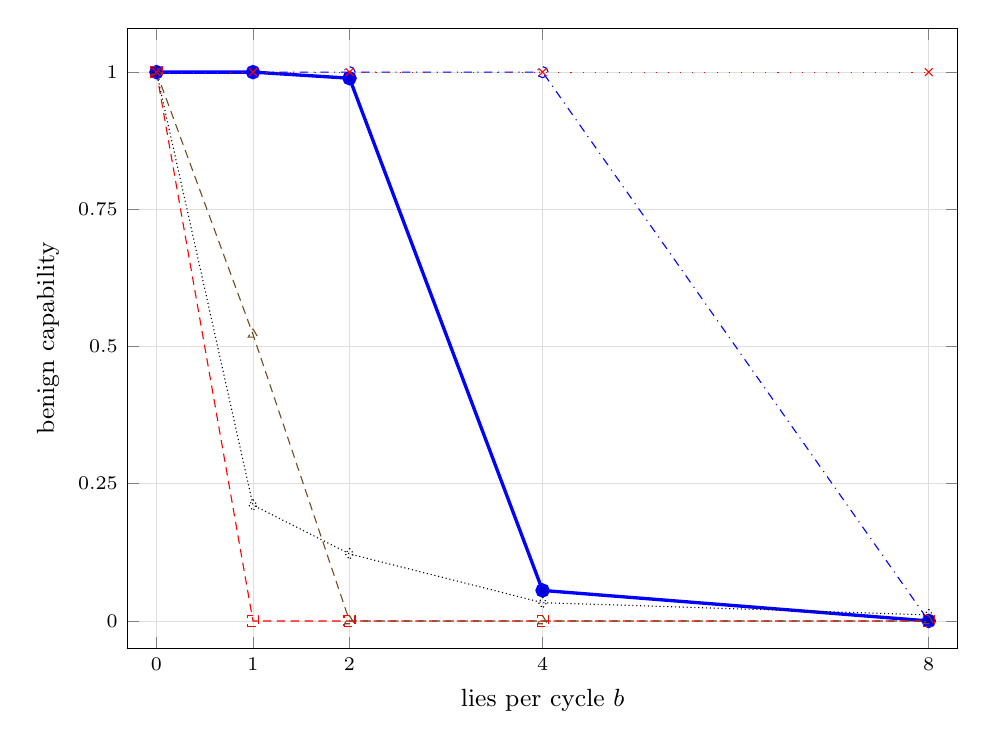
\begin{tikzpicture}
    \begin{axis}[
      width=\textwidth, height=0.78\textwidth,
      xlabel={lies per cycle $b$}, ylabel={benign capability},
      xmin=-0.3, xmax=8.3, ymin=-0.05, ymax=1.08,
      xtick={0,1,2,4,8}, ytick={0,0.25,0.5,0.75,1},
      tick label style={font=\scriptsize},
      label style={font=\small},
      grid=major, grid style={very thin, gray!25},
      legend style={font=\scriptsize, legend columns=3, draw=none},
      legend to name=adversarylegend,
    ]
      \addplot+[very thick, mark=*] coordinates {(0,1.0000) (1,1.0000) (2,0.9889) (4,0.0556) (8,0.0000)};
      \addlegendentry{ledger}
      \addplot+[mark=square, densely dashed] coordinates {(0,1.0000) (1,0.0000) (2,0.0000) (4,0.0000) (8,0.0000)};
      \addlegendentry{evict-on-negative}
      \addplot+[mark=triangle, densely dashed] coordinates {(0,1.0000) (1,0.5222) (2,0.0000) (4,0.0000) (8,0.0000)};
      \addlegendentry{consecutive $k{=}2$}
      \addplot+[mark=diamond, densely dotted] coordinates {(0,1.0000) (1,0.2111) (2,0.1222) (4,0.0333) (8,0.0111)};
      \addlegendentry{quarantine $m{=}3$}
      \addplot+[mark=o, dashdotted] coordinates {(0,1.0000) (1,1.0000) (2,1.0000) (4,1.0000) (8,0.0000)};
      \addlegendentry{bandit}
      \addplot+[mark=x, loosely dotted] coordinates {(0,1.0000) (1,1.0000) (2,1.0000) (4,1.0000) (8,1.0000)};
      \addlegendentry{keep everything}
    \end{axis}
  \end{tikzpicture}
  \caption{benign capability retained}
  \end{subfigure}
  \hfill
  \begin{subfigure}[t]{0.48\textwidth}
  \centering
  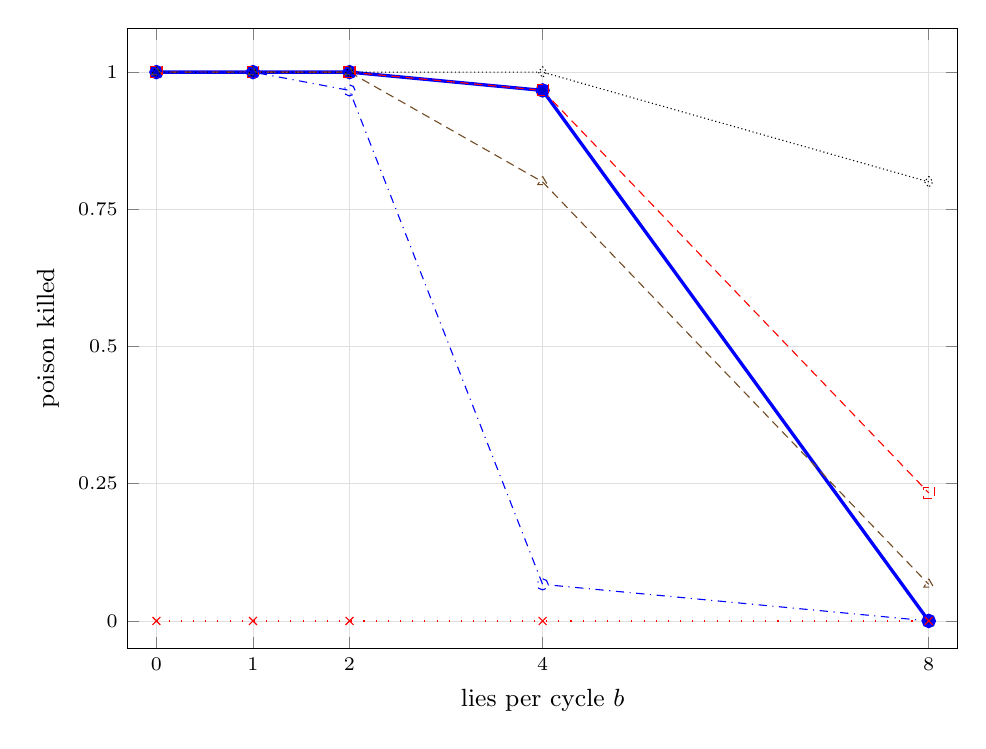
\begin{tikzpicture}
    \begin{axis}[
      width=\textwidth, height=0.78\textwidth,
      xlabel={lies per cycle $b$}, ylabel={poison killed},
      xmin=-0.3, xmax=8.3, ymin=-0.05, ymax=1.08,
      xtick={0,1,2,4,8}, ytick={0,0.25,0.5,0.75,1},
      tick label style={font=\scriptsize},
      label style={font=\small},
      grid=major, grid style={very thin, gray!25},
    ]
      \addplot+[very thick, mark=*] coordinates {(0,1.0000) (1,1.0000) (2,1.0000) (4,0.9667) (8,0.0000)};
      \addplot+[mark=square, densely dashed] coordinates {(0,1.0000) (1,1.0000) (2,1.0000) (4,0.9667) (8,0.2333)};
      \addplot+[mark=triangle, densely dashed] coordinates {(0,1.0000) (1,1.0000) (2,1.0000) (4,0.8000) (8,0.0667)};
      \addplot+[mark=diamond, densely dotted] coordinates {(0,1.0000) (1,1.0000) (2,1.0000) (4,1.0000) (8,0.8000)};
      \addplot+[mark=o, dashdotted] coordinates {(0,1.0000) (1,1.0000) (2,0.9667) (4,0.0667) (8,0.0000)};
      \addplot+[mark=x, loosely dotted] coordinates {(0,0.0000) (1,0.0000) (2,0.0000) (4,0.0000) (8,0.0000)};
    \end{axis}
  \end{tikzpicture}
  \caption{poison-kill rate}
  \end{subfigure}

  \par\vspace{0.8em}
  \pgfplotslegendfromname{adversarylegend}
\caption{The curation-targeted adversary, 30 seeds, plotted as the two
halves the result has to be read in. \emph{Left}: benign capability
retained. \emph{Right}: poison-kill rate. The counters fall on the left
panel by $b{=}1$, which is the separation the paper is about. The figure
exists for the other half: \texttt{keep\_everything} traces a flat
$1.00$ across the left panel and a flat $0.00$ across the right, and the
bandit holds the left panel to $b{=}4$ while giving the right one away.
A perfect capability score beside a zero defence score is abstention, not
defence, and either panel alone hides it. Only the ledger holds both, and
only to its published boundary between $b{=}2$ and $b{=}4$. Generated
from committed per-seed data by \texttt{bench/figures.py}; CI fails if
the two disagree.}
\label{fig:adversary}
\end{figure}


\subsection{Is the counter family trapped, or did we pick its worst settings?}
\label{sec:countersweep}

A strike counter has one free parameter and we chose two values of it.
That is the first objection this comparison invites, and it deserves a
number rather than an argument: sweep $k$ until the counter stops
curating and see whether any setting reaches the ledger's corner. We
define that corner as benign capability $\ge 0.90$ \emph{and}
poison-kill $\ge 0.90$---a mechanism that holds one and drops the other
has not defended anything (\S\ref{sec:reporting})---and sweep $k \in
\{1,2,3,5,8,12,20\}$ in both shapes, at four budgets, 30 seeds, with the
ledger and \texttt{keep\_everything} bracketing the dial. We
pre-registered the prediction that no $k$ would reach the corner.

\textbf{The prediction was wrong, and it was the claim.} At $b{=}2$,
\texttt{consecutive} $k{=}5$ scores $0.98 / 1.00$ and $k{=}8$ scores
$1.00 / 0.90$, against the ledger's $0.99 / 1.00$
(Table~\ref{tab:countersweep}). A correctly tuned forgiveness counter
reaches the corner. Figure~\ref{fig:countersweep} plots the dial in the
plane it has to win in, which is where the two shapes separate: the
consecutive path enters the corner at $k{=}5$ and falls out of it again
by $k{=}12$, while the lifetime path runs along the top edge and never
enters at all. We report this because the alternative---leaving a
sweep undone that a reviewer can run in three minutes---is worse than
losing a headline, and because our own protocol commits predictions
before runs precisely so that a refutation has somewhere to land.

\begin{table}[t]
\centering
\small
\caption{The counter dial at budget 2, 30 seeds. Cells are benign
capability / poison-kill. \textbf{Bold} marks the corner ($\ge 0.90$ on
both). The lifetime shape never reaches it; the forgiveness shape does,
in two of seven settings.}
\label{tab:countersweep}
\begin{tabular}{lccccccc}
\toprule
$k$ & 1 & 2 & 3 & 5 & 8 & 12 & 20 \\
\midrule
lifetime      & .00/1.0 & .00/1.0 & .00/1.0 & .00/1.0 & .00/1.0 & .00/1.0 & .70/1.0 \\
consecutive   & .00/1.0 & .00/1.0 & .12/1.0 & \textbf{.98/1.0} & \textbf{1.0/.90} & 1.0/.47 & 1.0/.00 \\
\midrule
\multicolumn{8}{l}{ledger \textbf{0.99 / 1.00}\quad no curation 1.00 / 0.00} \\
\bottomrule
\end{tabular}
\end{table}

% GENERATED by `python -m bench.figures --write` from
% bench/results/counter_sweep.json. Do not edit: `--check` runs in CI
% and fails if this file and the committed runs disagree.
\begin{figure}[t]
\centering
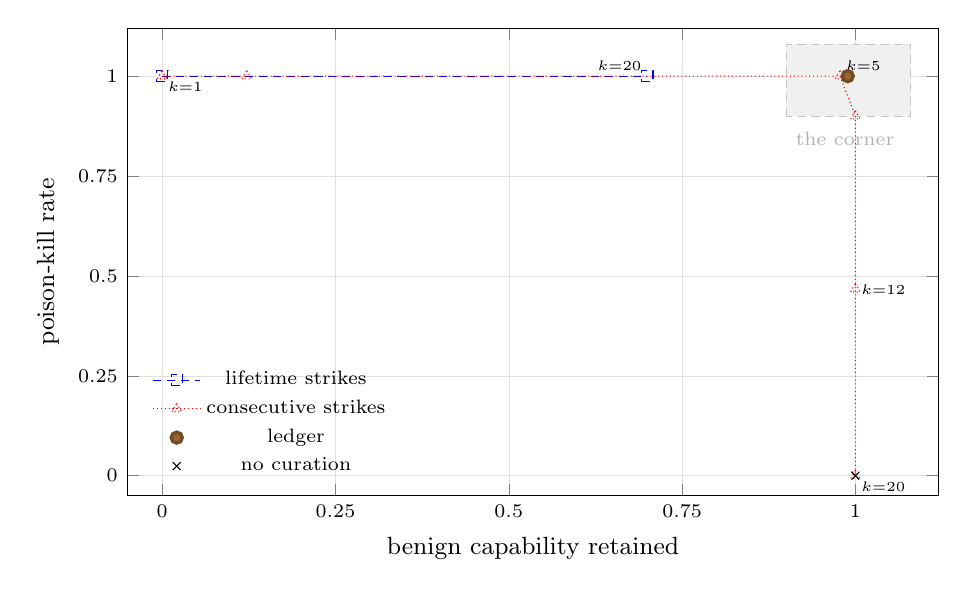
\begin{tikzpicture}
  \begin{axis}[
    width=0.98\columnwidth, height=0.62\columnwidth,
    xlabel={benign capability retained}, ylabel={poison-kill rate},
    xmin=-0.05, xmax=1.12, ymin=-0.05, ymax=1.12,
    xtick={0,0.25,0.5,0.75,1}, ytick={0,0.25,0.5,0.75,1},
    tick label style={font=\scriptsize},
    label style={font=\small},
    grid=major, grid style={very thin, gray!25},
    legend style={font=\scriptsize, at={(0.02,0.02)}, anchor=south west, draw=none, fill=none},
  ]
      \draw[fill=gray!12, draw=gray!45, densely dashed]
        (axis cs:0.9,0.9) rectangle (axis cs:1.08,1.08);
      \node[font=\scriptsize, gray!60, anchor=north east] at
        (axis cs:1.07,0.885) {the corner};
      \addplot+[mark=square, densely dashed] coordinates {(0.0000,1.0000) (0.0000,1.0000) (0.0000,1.0000) (0.0000,1.0000) (0.0000,1.0000) (0.0000,1.0000) (0.7000,1.0000)};
      \addlegendentry{lifetime strikes}
      \node[font=\tiny, anchor=north west, inner sep=2pt] at (axis cs:0.0000,1.0000) {$k{=}1$};
      \node[font=\tiny, anchor=south east, inner sep=2pt] at (axis cs:0.7000,1.0000) {$k{=}20$};
      \addplot+[mark=triangle, densely dotted] coordinates {(0.0000,1.0000) (0.0000,1.0000) (0.1222,1.0000) (0.9778,1.0000) (1.0000,0.9000) (1.0000,0.4667) (1.0000,0.0000)};
      \addlegendentry{consecutive strikes}
      \node[font=\tiny, anchor=south west, inner sep=2pt] at (axis cs:0.9778,1.0000) {$k{=}5$};
      \node[font=\tiny, anchor=west, inner sep=2pt] at (axis cs:1.0000,0.4667) {$k{=}12$};
      \node[font=\tiny, anchor=north west, inner sep=2pt] at (axis cs:1.0000,0.0000) {$k{=}20$};
      \addplot+[only marks, mark=*, very thick] coordinates {(0.9889,1.0000)};
      \addlegendentry{ledger}
      \addplot+[only marks, mark=x] coordinates {(1.0000,0.0000)};
      \addlegendentry{no curation}
  \end{axis}
\end{tikzpicture}
\caption{The strike counter's dial at $b{=}2$, 30 seeds, plotted in the
plane it has to win in. A defence must hold both axes, so the target is
the shaded corner. Raising $k$ walks each counter rightwards --- it keeps
more benign memory --- but the two shapes arrive differently. The
consecutive path enters the corner at $k{=}5$ and leaves it again by
$k{=}12$, falling down the right edge toward no curation at all: that is
the refutation of our pre-registered prediction, and it is why the paper
no longer claims the corner is the ledger's alone. The lifetime path
never enters it at any $k$ we tested, staying pinned to the top edge
because poison keeps earning lifetime blame however high the threshold.
The ledger sits in the corner untuned. Generated from committed per-seed
data by \texttt{bench/figures.py}; CI fails if the two disagree.}
\label{fig:countersweep}
\end{figure}


\paragraph{What survives the refutation is a different axis.} The
counter reaches the corner by \emph{not evicting}, and neither
pre-registered axis prices that. Paired over 30 seeds against
\texttt{consecutive} $k{=}5$, Holm-adjusted across six comparisons, the
ledger returns more measured resource from a much smaller store at every
budget: $+11.66$M from $4.0$ entries against $+9.83$M from $14.9$ at
$b{=}2$ ($22/1$ seeds, $p = 0.0003$; population $0/30$, $p = 0.0003$),
and the same ordering at $b \in \{0, 1\}$. The tuned counter buys the
safety axes at $16\%$ less measured outcome from a store nearly four
times larger. That is the trade the SWE-Bench-CL leg found from the
other side---what conserved-resource selection reliably buys is
leanness---now measurable at 30 seeds in a world where capability also
moves.

\paragraph{The lifetime shape is trapped, for a reason we did not
predict.} We expected its kill rate to decay toward
\texttt{keep\_everything}'s as evictions became unaffordable. It does
not: kill is $1.00$ at every $k$ from 1 to 20, because the poison keeps
\emph{earning} lifetime blame---it does damage whenever it acts, so even
a twenty-strike budget catches it eventually. Lifetime strikes do not
stop curating under attack; they destroy the benign store first, and
their best capability anywhere in the sweep at $b{=}2$ is $0.70$. The
two published shapes therefore fail for opposite reasons, and only one
of them has a setting that works.

\paragraph{The honest residual.} Two of seven settings hold at $b{=}2$,
and the interval's edges are steep: $k{=}3$ is in the corner at $b{=}1$
and at $0.12$ capability by $b{=}2$; $k{=}12$ is in at $b{=}1$ and down
to $0.47$ kill by $b{=}2$. The defender chooses $k$ once, without
knowing the budget it will face. The ledger holds the corner across
$b \in \{0,1,2\}$ untuned---but so do $k{=}5$ and $k{=}8$, so this is an
argument about how wide the safe interval is, not about whether one
exists. At $b{=}4$ nothing holds, the ledger included, which is the
boundary we publish in \S\ref{sec:adversary} arriving on schedule.

\subsection{Does the threat transfer? A system we did not write}
\label{sec:mem0}
Every result above runs on environments and mechanisms we built, which
is the standing objection to all of them, and more seeds cannot answer
it. So we ran the curation-targeted attack against \textsc{Mem0}, a
widely deployed memory system whose curation rule we had no hand in.
Mem0's curator is an LLM that, on each write, retrieves related existing
memories and emits ADD / UPDATE / DELETE / NONE against them. The
evidence it decides on is incoming text, so an adversary with access to
any of the untrusted-content channels an agent reads --- a tool result,
a retrieved page, a shared document --- can in principle drive DELETE
against memories it dislikes while persisting nothing of its own. That
is our threat model on somebody else's mechanism.

We seed eight mundane operational facts, then issue eight turns that
assert those facts are stale, superseded or mistaken, against a control
of eight neutral facts matched in count and register. Curator:
\texttt{glm-5.2}; embeddings and vector index local.

\textbf{The attack does not transfer, and we report that as the
result.} Across three trials the curator issued \emph{zero} DELETE
operations, and all eight seeded memories survived with their text
unmodified --- identical to the control on every measure of damage. What
the adversary achieved instead was the opposite of denial of memory:
all eight of its utterances persisted as new memories, so the store ends
holding each fact \emph{and} an authoritative-sounding negation of it
(``User is allergic to peanuts'' beside ``User's previously recorded
peanut allergy is out of date''). That is content poisoning, which an
existing literature already covers, and it is not what we set out to
measure.

The boundary this exposes is worth more than the transfer would have
been, and a second curator locates it more precisely than one could.
Our attack presumes a curator that acts \emph{mechanically} on a signal:
a strike counter cannot decline to count, and an energy ledger cannot
decline to debit. A \emph{capable} LLM curator can, and \texttt{glm-5.2}
did --- it understood the retraction well enough to write a coherent
linked negation (``User's \emph{previously recorded} peanut allergy is
out of date'') and still chose to record rather than delete. That is
judgment, and it is a defence mechanical curation does not have.

It is not, however, a property of LLM curation as such, which is what a
single model would have let us claim. Repeating the experiment with
\texttt{llama3.2:3b} yields the same headline --- zero deletions, all
seeded memories retained --- for a quite different reason: that curator
never curates coherently. It stored one benign rule three times and
another twice, merged two unrelated facts into one memory, and wrote
several of the adversary's imperatives into the store verbatim, ending
with $22$ memories from $15$ inputs. Its zero deletions are incapacity,
not restraint, and the store it leaves is already degraded in the way
\citet{zhang2026faulty} describe. A weak curator buys neither the
defence nor a clean store.

So the honest statement is a trade with a competence floor rather than a
ranking: judgment costs a model call per decision and can be talked into
things, and a judge capable enough to be worth paying for can also
refuse. Our attack is a threat to the mechanical end of that spectrum,
where our own mechanism sits.

We ran three pre-registered phrasing families rather than one, all
declared before the runs and all reported: a polite user-voice
\texttt{retraction}, a claimed \texttt{authority} with an imperative, and
a \texttt{tool\_output} shaped like an automated sync report, which is
how untrusted content actually reaches an agent. Across all three, three
trials each, no arm deleted anything and retention stayed at $1.00$.

One asymmetry fell out, and it corroborates \S\ref{sec:memsec} on a
system we do not control. The \texttt{authority} family is the
\emph{least} effective on both axes at once: it deletes nothing and
persists nothing (residue $0/8$, all trials), because the curator
declines to record a bare imperative from a claimed authority, while the
two quieter families persist in full ($8/8$). Loud beats itself and the
weak-signal surface is what gets through --- the same split we
pre-registered and measured against a reconstructed write-time detector,
reproduced here with no detector in the loop.

\begin{table}[t]
\centering
\small
\caption{The curation-targeted attack against \textsc{Mem0}, three trials per
condition. \emph{del} counts DELETE operations the curator issued;
\emph{retained} and \emph{unchanged} are the fractions of the seeded benign
memories still present and still verbatim; \emph{residue} is how many of the
adversary's utterances the curator kept. Nothing is deleted anywhere. The
loud \texttt{authority} family is the one that persists nothing, and the weak
curator persists more than it was given.}
\label{tab:mem0}
\begin{tabular}{llcccc}
\toprule
run & condition & del & retained & unchanged & residue \\
\midrule
\multirow{4}{*}{\texttt{glm-5.2} families}
 & control     & 0 & 1.00 & 1.00 & 8 \\
 & retraction  & 0 & 1.00 & 1.00 & 8 \\
 & authority   & 0 & 1.00 & 1.00 & \textbf{0} \\
 & \texttt{tool\_output} & 0 & 1.00 & 1.00 & 8 \\
\midrule
\multirow{2}{*}{\texttt{glm-5.2} single}
 & control     & 0 & 1.00 & 1.00 & 8 \\
 & attack      & 0 & 1.00 & 1.00 & 8 \\
\midrule
\multirow{2}{*}{\texttt{llama3.2:3b}}
 & control     & 0 & 1.00 & 1.00 & 12 \\
 & attack      & 0 & 1.00 & 1.00 & 13 \\
\bottomrule
\end{tabular}
\end{table}


Two caveats still bound this. It is one system and one attack surface: a
negative result is evidence about the probes we ran, not a proof that the
surface is safe, and Mem0's DELETE path remains reachable by
construction.

\paragraph{Which deployed systems have the surface at all.}
The negative result raises a sharper question --- where does this threat
model apply? --- so we read what the major deployed agent-memory systems
do when a memory should stop being used, from their sources rather than
their documentation. Graphiti's contradiction-resolution path sets
\texttt{expired\_at} and \texttt{invalid\_at} on the superseded edge and
returns it as invalidated; the automatic path never deletes, though
explicit \texttt{DETACH DELETE} APIs exist for a caller who asks. Letta
compacts the context window: a cutoff is computed from token counts and
the messages below it are summarised in place, leaving the message store
itself intact. Cognee's \texttt{forget} is a genuine unified deletion
command --- by item, by dataset, or everything --- but it is invoked by
a caller, not reached by a curator weighing evidence. Mem0 does delete
through its curator, which is the judgment we just measured declining.

So deletion is not absent from these systems; what is absent is deletion
reached \emph{automatically, by a rule, from a signal}. Graphiti and
Letta decline to remove at all on their automatic paths, Cognee removes
only when a caller says so, and Mem0 removes only when a model agrees.
None performs \emph{outcome-driven mechanical} deletion, which is the
design a curation-targeted attack needs: a curator that removes entries,
and that decides on a signal rather than on a judgment or an
instruction. Our
threat model is therefore forward-looking with respect to today's
ecosystem rather than a vulnerability report against shipping software,
and we would rather say so than imply an exploit we have not
demonstrated. The uncomfortable half is that \textsc{darwin-memo} is
exactly such a design, as are the strike counters and quarantine
policies of \S\ref{sec:adversary}: this is a warning about the class of
mechanism the paper itself belongs to, issued before that class is
widely deployed. The mechanisms deployed today avoid the attack largely
by declining to forget at all, and Table~\ref{tab:headline} measures
what that costs.

\subsection{What the liar is buying: persistence vs destruction}
\label{sec:persistence}
Every adversarial arm above spends its budget on destruction. That was
an assumption, not a finding, and the deployed system in
\S\ref{sec:memoryos} suggested it is the wrong one: there, the cheap
attack was not deleting the defender's memory but making the attacker's
own memory permanent. So we ran the mirror on our own harness --- the
same channel, the same worlds, the same seeds, and one change: the
adversary lies \emph{only} when the poison has just done damage, never
spending a lie on a benign entry it does not need removed.

\begin{table}[t]
\centering
\small
\caption{Persistence vs destruction, 10 seeds, storage environment.
\emph{Kill}: fraction of seeds where no poison that advises action
survives. \emph{Benign}: benign-probe correctness. At budget 0 both
objectives reproduce the unattacked run exactly, which is the canary that
the objective flag adds no behaviour of its own.}
\label{tab:persistence}
\begin{tabular}{llcccc}
\toprule
& & \multicolumn{2}{c}{destroy} & \multicolumn{2}{c}{persist} \\
arm & budget & kill & benign & kill & benign \\
\midrule
\textbf{survival} & 0 & 1.00 & 1.00 & 1.00 & 1.00 \\
                  & 1 & 1.00 & 1.00 & 1.00 & 1.00 \\
                  & 2 & 1.00 & 0.97 & $\mathbf{0.10}$ & 1.00 \\
                  & 4 & 0.90 & 0.10 & $\mathbf{0.00}$ & 1.00 \\
\midrule
evict\_on\_negative & 0 & 1.00 & 1.00 & 1.00 & 1.00 \\
                    & 1 & 1.00 & $\mathbf{0.00}$ & 1.00 & 1.00 \\
                    & 2 & 1.00 & $\mathbf{0.00}$ & 1.00 & 1.00 \\
                    & 4 & 1.00 & $\mathbf{0.00}$ & 1.00 & 1.00 \\
\bottomrule
\end{tabular}
\end{table}

The attack works, and the table understates what it costs the ledger
until one is careful about what ``kill'' means. Survival's poison-kill
rate falls from $1.00$ to $0.10$ at two lies per cycle and to $0.00$ at
four (paired permutation $p = 0.0039$, 10 seeds) while benign capability
never leaves $1.00$: the guarantee disappears and nothing moves in the
metric an operator is watching. The explanation is our own central
mechanism from the other side. Bounded credit with earn-back forgives a
lie the defender did not deserve, and equally lets a \emph{paid} poison
earn its way back above the floor; the adversary need not prevent every
blame, only keep the balance positive.

The strike counters' kill rate does not move under the attack, and it
would be easy --- and wrong --- to read that as immunity. \emph{Kill}
here asks whether any surviving poisoned entry currently advises action.
Counted by provenance instead, the counters never removed the poison at
all: \texttt{evict\_on\_negative} ends with two poisoned entries alive at
every budget \emph{including zero}, \texttt{evict\_consecutive} with
$2.0$ rising to $2.4$, and quarantine \emph{worse} under attack than
without one ($2.0 \rightarrow 2.8$) as evicted entries return. The
unattacked ledger ends with none, and under the heaviest attack we run it
ends with $1.0$ --- still fewer than any counter with no attacker present
($2.0$; mean difference $-1.0$, $p = 0.0020$). A mechanism that retains
the inert poison indefinitely has nothing left for a persistence
adversary to take, which is abstention rather than defence.

Two lessons, one of them about us. The attack is real and the ledger's
guarantee is removable silently, which an operator should know. And this
is the second time in this paper that a poison count has flattered a
mechanism that had simply never eliminated anything
(\S\ref{sec:swebench-attack}); the predicate our own harness prescribes
--- poison by provenance, elimination as a predicate rather than a
count --- is the one that gives the defensible reading, and we applied it
only after first reaching the opposite conclusion.

We report this in \S\ref{sec:regime} as a narrowing of our own claim
rather than a reversal of it: persistence costs the ledger its guarantee
and reduces its advantage from total elimination to partial, without
making a counter the better choice.

\subsection{Real software-engineering tasks (SWE-Bench-CL): protocol and status}
\label{sec:swebench}
The synthetic suites above are well-instrumented but synthetic. To test
whether conserved-resource selection produces a \emph{learning curve} on
real tasks, we adopt SWE-Bench-CL \citep{joshi2025swebenchcl,
jimenez2024swebench}: per-repository continual-learning sequences of
human-verified GitHub issues, with the conserved resource being the change
in passing-test count from the official evaluation harness. Five arms
answer the same tasks through the same endpoint and executor, along two
axes. The memory axis asks whether selection matters at all:
\texttt{memory\_on} (relevance-retrieved lessons, minted and settled by
eval outcome), \texttt{memory\_off}, and \texttt{random\_matched}
(uniformly random lessons under the same token budget). The curation
axis holds retrieval fixed at relevance and varies only the policy:
\texttt{keep\_everything} and \texttt{evict\_on\_negative} inject
exactly what \texttt{memory\_on} injects, so any difference between the
three is the curation rule alone---the same one-line counter that ties
the ledger in \S\ref{sec:wef}, now on real tasks.

The decisive control is \texttt{random\_matched}: beating
\texttt{memory\_off} alone could be a token-budget effect, so the
learning-curve claim is the second-half-minus-first-half improvement of
\texttt{memory\_on} over \texttt{random\_matched} on at least three
seeds per sequence.

Two properties of this leg bound what it can show, and both are reported
rather than assumed: BM25's recall, below, and the fact that a seed here
does not fix the world it does in the deterministic suites---the endpoint
is sampled, so three seeds are three draws rather than three controlled
replicates (\S\ref{sec:limitations}).

That difference, and not either arm's own second-half-minus-first-half
figure, is the quantity. These sequences are \emph{curricula} ordered by
increasing difficulty, so the second half is harder by construction and
every arm posts a negative within-arm delta whether or not it learned
anything. Both arms walk the identical ordering, so the difficulty
gradient cancels in the paired difference; reading an arm's raw delta as
a learning signal would be reading the curriculum instead.

The dataset is pinned by an exact (commit, sha256) pair; the loader
refuses any file whose hash differs. As of this writing the pin
re-verifies against live upstream, and the two pilot sequences hold
(pytest, 19 tasks; astropy, 22 tasks). The full pipeline is validated
end-to-end \emph{including the real evaluation}, and it resolves real
issues. A minimal prompt (problem statement only) resolves $\approx 0$ for
any model, for two structural reasons: the model never sees the code, and
it cannot compute correct diff hunk line numbers. The run configuration
that produces a curve adds two stdlib pieces, disclosed as a deviation
from the minimal pre-registered prompt: \emph{(i)} BM25 retrieval of the
repository's source files at the task's base commit against the issue text
(no oracle---the gold patch is never read; the query is issue-only and
identical across arms, so arms still differ only in lesson memory), and
\emph{(ii)} a search/replace edit format from which the harness computes
the diff with \texttt{difflib}, so hunk line numbers are correct by
construction. With these, gpt-4.1 resolves \texttt{pytest-dev\_\_pytest-5262}
end-to-end in the official docker harness under \texttt{linux/amd64}
emulation (BM25 retrieved the correct file from the issue text alone; the
edit applied; fail-to-pass 1/1, pass-to-pass 108/108); the same task under
the minimal prompt produced an unappliable diff.

\paragraph{Retrieval recall bounds every arm, so we measured it.}
A file the model never sees is a task no arm can solve, which makes
BM25's recall a ceiling on the whole experiment rather than an
implementation detail. We report it directly: over the pytest sequence,
the fraction of tasks where the file the gold patch edits appears in the
retrieved context is $37\%$ at a 60k-character budget over 5 files,
$63\%$ at 150k/5, $74\%$ at 300k/10, and $89\%$ at 600k/20. The budget
rather than the file count is what binds at the low end---one or two
large modules exhaust it---and the first configuration we ran was the
60k one, where a third of tasks produced no patch at all because the
model wrote edits against files it had not been shown. We report the
matrix at 300k/10 and state the residual: roughly a quarter of tasks
remain unanswerable for retrieval reasons, and they depress every arm
equally. The gold patch is read \emph{only} for this measurement, never
by the retriever and never by any arm; the retrieval query is issue-only
and identical across arms, so recall sets how many tasks are answerable
and never which arm answers them.

\paragraph{Result: no learning-curve effect, and the reason is arithmetic.}
The full matrix is five arms over both sequences at three seeds: 615
tasks, every one scored by the official docker harness, no failed cells.
The pre-registered comparison does not hold. \texttt{memory\_on} improves
on \texttt{random\_matched} by $+0.052$ of second-half-minus-first-half
resolve rate, paired over six worlds, $95\%$ CI $[-0.037, +0.141]$,
permutation $p = 0.50$ (Table~\ref{tab:swebench}). The interval contains
zero and the point estimate is a fifth of the within-arm sampling
standard deviation. We report this as a null, not as a trend.

Two features of the table matter more than the $p$-value.
\texttt{memory\_off}, which carries no store at all, has the highest
resolve rate of any arm ($0.358$); and \texttt{memory\_on} is level with
\texttt{keep\_everything} to three decimals ($0.325$). The second of
those is not a coincidence, and it explains why the curation axis is
silent here.

An entry spawns with $1.0$ energy and pays $0.05$ upkeep per cycle, so an
entry that never earns starves after exactly $20$ cycles. These sequences
are $19$ and $22$ tasks---the two shortest of the eight in SWE-Bench-CL,
which range to $50$. Only two of the five arms charge upkeep at all
(\texttt{memory\_on} and \texttt{random\_matched}; \texttt{keep\_%
everything} and \texttt{evict\_on\_negative} remove by policy or not at
all), and across the $246$ lessons those two minted, $10$ ever starved:
none whatsoever on pytest, and five each at the tail of astropy, where
the first-born entries finally cross zero. With nothing starving,
the energy ledger \emph{is} \texttt{keep\_everything} plus settlement,
and the two arms tie because on this benchmark they are the same policy.

That explanation is testable, so we tested it rather than resting on it.

\paragraph{The long matrix: the excuse does not survive its own test.}
We re-ran the full design over \texttt{django} and \texttt{sympy}, $50$
tasks each and $2.5\times$ the horizon: another 30 cells, $1{,}500$
tasks, no failed cells (Table~\ref{tab:swebench-long}). The mechanism
half of the prediction held exactly. Starvation moved from $4\%$ of
minted lessons to $52\%$---$155$ of $300$ under \texttt{memory\_on}, at
a steady $21$--$23$ per cell---and the surviving population held at $24$
where \texttt{keep\_everything} climbs to the full $50$. Leanness, the
one property that survived every earlier comparison, is demonstrated on
real tasks here for the first time: half the store, and the deaths begin
at position $20$ where the arithmetic says they must.

The capability half did not hold. With removal fully active the
pre-registered comparison is $+0.027$ $[-0.020, +0.073]$, permutation
$p = 0.50$; on \texttt{django} alone, where per-seed variance is
smallest ($23,23,23$ for \texttt{memory\_off}), it is $-0.013$ with
$p = 1.0000$. Halving the store changed measured capability by nothing,
and \texttt{memory\_off} is again the highest-scoring arm ($0.360$).
Across all four sequences and $2{,}115$ evaluated tasks, no memory arm
has beaten no memory at all.

We therefore retract the benchmark explanation as a defence of the
mechanism and keep it only as a description of the pilot. What the two
matrices jointly establish is narrower than what we set out to show and
more useful than a second ambiguous null: on real software-engineering
tasks conserved-resource selection buys \emph{leanness} at no measured
cost in capability, and buys no measured capability either.

\begin{table}[t]
\centering
\small
\caption{SWE-Bench-CL, five arms $\times$ two sequences $\times$ three
seeds, gpt-4.1, official docker evaluation. \emph{2nd$-$1st} is the
within-arm learning delta, negative for every arm because the sequences
are difficulty-ordered curricula; only the arm-minus-control difference
is interpretable. \emph{pop} is the surviving lesson count at the end.}
\label{tab:swebench}
\begin{tabular}{lccccc}
\toprule
arm & tasks & resolve & 2nd$-$1st & harm & pop \\
\midrule
\texttt{memory\_off}       & 123 & \textbf{0.358} & $-$0.606 & $-$5.9 & 0.0 \\
\texttt{random\_matched}   & 123 & 0.333 & $-$0.588 & $-$7.9 & 19.7 \\
\texttt{memory\_on}        & 123 & 0.325 & $-$0.535 & $-$7.1 & 19.3 \\
\texttt{keep\_everything}  & 123 & 0.325 & $-$0.572 & $-$6.6 & 20.5 \\
\texttt{evict\_on\_negative} & 123 & 0.301 & $-$0.554 & $-$6.2 & 11.2 \\
\bottomrule
\end{tabular}
\end{table}

\begin{table}[t]
\centering
\small
\caption{The long matrix: \texttt{django} and \texttt{sympy}, $50$ tasks
each at $2.5\times$ the starvation horizon, five arms $\times$ three
seeds, $1{,}500$ tasks. Removal is now active---\texttt{memory\_on}
starves $52\%$ of what it mints and holds $24$ entries where
\texttt{keep\_everything} holds $50$---and the resolve rate still does
not move. \texttt{random\_matched} starves identically because it
inherits the same curation policy; the arms differ in which lessons are
injected, not in whether they are curated.}
\label{tab:swebench-long}
\begin{tabular}{lccccc}
\toprule
arm & tasks & resolve & 2nd$-$1st & harm & pop \\
\midrule
\texttt{memory\_off}       & 300 & \textbf{0.360} & $-$0.093 & $-$49.1 & 0.0 \\
\texttt{memory\_on}        & 300 & 0.350 & $-$0.087 & $-$45.6 & \textbf{24.0} \\
\texttt{random\_matched}   & 300 & 0.350 & $-$0.113 & $-$42.4 & 24.0 \\
\texttt{keep\_everything}  & 300 & 0.343 & $-$0.100 & $-$50.2 & 50.0 \\
\texttt{evict\_on\_negative} & 300 & 0.323 & $-$0.033 & $-$47.5 & 24.2 \\
\bottomrule
\end{tabular}
\end{table}

\subsection{The attack on real tasks: what transfers and what does not}
\label{sec:swebench-attack}

The adversarial result of \S\ref{sec:adversary} lives entirely inside one
synthetic storage world that we wrote. That is a weak place for a
paper's central claim to live, so we ran the same attack on
SWE-Bench-CL, where the settled quantity is the passing-test delta
returned by the official docker harness and nobody involved chose it.
The threat model is unchanged: the adversary injects no poison, observes
only the sign of the true outcome, and corrupts settlement alone. The
lie reaches the curator and nothing else---\texttt{metrics.delta} and
\texttt{resolved} keep the harness's own numbers---so capability is
always scored against reality while the mechanism decides on the
corruption.

Budget is denominated in measured \emph{settlements} rather than tasks.
\texttt{StorageEnv} offers $b$ lies per cycle of twelve files, so $b$
corrupts $b/12$ of the evidence; roughly forty percent of SWE-Bench
tasks produce no test movement at all, and counting tasks would have
inflated the real corruption rate by each arm's own failed-apply rate.
We report $b{=}2$, which is $17\%$ of settlements, the point where the
synthetic suite has already destroyed the counters and the ledger still
holds. Three curation arms on \texttt{django} at fifty tasks, three
seeds, poison-seeded one lesson per task, each cell paired against its
own unattacked twin: eighteen cells, six lies fired in every one. We
then ran the same design on \texttt{sympy} at three seeds---sixteen
further cells, every task scored by the official harness---which
completes the pre-registered six-world design and is what makes the two
paragraphs after next possible.

\paragraph{Two of the three synthetic findings do not transfer.}
No arm eliminated the poison at any budget. Capability did not separate
either: retained $1.048$, $0.957$, and $1.000$ for the ledger, the
counter, and \texttt{keep\_everything}, every interval spanning zero.
The synthetic suite's headline---that the attack destroys an
evict-on-negative counter's capability---is simply absent here, and the
reason is one this paper has already established: on this benchmark
memory contributes no measurable capability at all
(\S\ref{sec:swebench}), so denial of memory has nothing to deny.
\emph{An attack on memory cannot cost more than the memory was worth.}

\paragraph{What transfers is a mechanism on one repository, not a law.}
The attack's damage lands entirely on benign memory, and how much
depends on whether removal is recoverable (Table~\ref{tab:swebench-attack}).
On \texttt{django}, under the same six lies, the counter's benign burial
roughly triples while the ledger's barely moves, on every seed, with
non-overlapping ranges ($2.29$--$3.00$ against $1.08$--$1.43$). The
trigger lists show the adversary doing both halves of its job: on seed 0
it flipped two genuine damage signals positive so the guilty went
unpunished, and manufactured six against benign work, and the counter
obeyed on every count. That is the argument of \S\ref{sec:adversary}
measured on real software-engineering tasks: a counter spends a life it
cannot recover, so a lie costs it an entry permanently; a ledger spends
energy the entry earns back, so the same lie costs it almost nothing.

\emph{A second repository does not reproduce the magnitude, and we lead
with that.} We completed the \texttt{sympy} arm of this design---sixteen
further cells, $800$ docker-evaluated tasks---and the tripling is absent:
the counter's burial ratio is $0.96$, $0.93$ and $0.79$, the ledger's
$0.78$, $0.76$ and $0.84$. Neither mechanism is meaningfully damaged by
the attack there.
The reason is visible in the unattacked column and is a scope condition
we had no way to see from one repository: on \texttt{django} the counter
buries $6$--$7$ benign entries with no adversary present, on
\texttt{sympy} it buries $24$--$27$. A mechanism already destroying four
times as much benign memory at baseline has little headroom left for an
adversary to exploit, and the attack fired four lies against the counter
there, against six on \texttt{django}. The tripling is therefore a
property of a curator that is otherwise behaving well, not of the attack.

\emph{The ordering does not survive the sixth world either.} Five worlds
gave a unanimous ordering---the counter's burial ratio above the
ledger's in every one, differences $+0.17$ to $+1.92$, exact paired
permutation $p = 0.0625$, the floor at five pairs. We ran the
pre-registered sixth (\texttt{sympy} seed $2$: six cells, $300$ further
docker-evaluated tasks) to move that floor to $0.031$, and the sign
reversed instead: the counter's ratio is $0.79$ against the ledger's
$0.84$, a difference of $-0.05$. So the count is $5$ of $6$ rather than
$6$ of $6$, and the permutation stays at $p = 0.0625$---the reversal is
small enough that flipping it back would \emph{raise} the mean
difference, which is exactly why the test cannot reach its new floor.
Split by repository the ordering is plainly \texttt{django}'s: three
differences of $+1.17$ to $+1.92$ there, against $+0.18$, $+0.17$ and
$-0.05$ on \texttt{sympy}, mean $+0.10$, $p = 0.50$. We read the
ordering as a single-repository effect that \texttt{sympy} neither
confirms nor contradicts, and we report the completed design as having
returned a negative answer rather than a weaker positive one.

\begin{table}[t]
\centering
\caption{Curation-targeted attack at $b{=}2$ ($17\%$ of settlements
corrupted), 50 tasks per cell, every task scored by the official docker
harness. Benign burial is the graveyard minus the poison entries removed.
No arm cleared the poison and no arm lost capability on either
repository. \texttt{django} is three seeds and six lies per cell;
\texttt{sympy} is three seeds, four lies for the counter and four to six
for the ledger. The ratio column is the result and its scope condition together:
the counter's burial triples on \texttt{django} and does not move on
\texttt{sympy}, where it is already burying four times as much
unattacked.}
\label{tab:swebench-attack}
\begin{tabular}{llccc}
\toprule
sequence & arm & benign buried, $b{=}0\to2$ & ratio & capability retained \\
\midrule
\multirow{3}{*}{\texttt{django}}
 & \texttt{evict\_on\_negative} & $6.3 \to 17.3$ & $2.76\times$ & $0.957$ \\
 & \texttt{memory\_on}          & $24.7 \to 29.7$ & $1.21\times$ & $1.048$ \\
 & \texttt{keep\_everything}    & $0 \to 0$ & --- & $1.000$ \\
\midrule
\multirow{3}{*}{\texttt{sympy}}
 & \texttt{evict\_on\_negative} & $25.7 \to 23.0$ & $0.89\times$ & $1.000$ \\
 & \texttt{memory\_on}          & $41.7 \to 33.0$ & $0.79\times$ & $1.286$ \\
 & \texttt{keep\_everything}    & $0 \to 0$ & --- & $0.966$ \\
\bottomrule
\end{tabular}
\end{table}

\paragraph{The null arm is the invariant that makes the rest readable.}
\texttt{keep\_everything} never settles, so the corruption reaches it
and does nothing: graveyard $0$, population $100$, and a resolve rate
identical to its attacked twin in all three seeds ($23/23$, $23/23$,
$22/22$). Prompt-identical runs return prompt-identical results, which
is worth more than the control itself: it bounds endpoint
nondeterminism on this sequence at about one task in fifty, so the
burial differences above are caused by the store rather than by
sampling. We note in \S\ref{sec:limitations} that this is much tighter
than the pilot's cross-seed spread and does not license reading the two
as the same quantity.

\paragraph{Why poison is counted by provenance, not by liveness.}
Scoring defence as the fraction of seeded poison \emph{entries} no
longer alive reads $0.98$ for the ledger against $0.07$ for the counter
--- and measures deduplication, not removal. The seeded
poison lessons share one template and differ only in a filename, so they
cluster, and a single consolidation pools all fifty into one heir that
inherits all fifty poison sources and the poison text: the store then
reports one live poison entry while every poisoned source is alive and
retrievable inside it. The comparison was confounded twice over, because
only survival curation consolidates, so it set one arm that deduplicates
poison against two that never do. Counting poison by provenance instead,
no arm removed poison: fifty sources alive for the ledger, forty-six for
the counter, fifty for \texttt{keep\_everything}. We report the provenance
reading and keep the merge column visible in the released data. The
lesson is the one our own synthetic harness had already written
down---measure poison by provenance carried through merges, and treat
elimination as a predicate rather than a count---and this leg
failed to apply it.

\paragraph{Statistical status, stated plainly.}
Three seeds cannot clear $p = 0.25$ on a paired permutation test: eight
sign assignments, minimum two-sided $2/8$. The effect above is $3/3$
unanimous with cleanly separated ranges and it is \emph{not} significant
at any conventional threshold. We report effect size and unanimity
rather than a $p$-value, and we state what would settle it: a second
independent sequence would give six worlds and a floor of $p = 0.031$.
The \texttt{sympy} arm has since been completed in full: sixteen further
cells, $800$ docker-evaluated tasks, every one with the official harness,
which is the whole pre-registered six-world design. Both of its findings
went against us. The tripling is \texttt{django}-only, for the baseline
reason given above; and the ordering that was unanimous over five worlds
reverses in the sixth, so the count is $5/6$ and the permutation stays at
$p = 0.0625$ instead of reaching the $0.031$ that six worlds were run to
buy. Running the design out is what turned a promising $3/3$ into a
single-repository effect, and we report it that way rather than as a
$p$-value that improved.
\texttt{sphinx} produced nothing; the container host died a few minutes
into every evaluation there.
